\documentclass[11pt,letterpaper,notitlepage]{article}

%================== Document nomenclature
\newcommand{\DOCSUBJT}{Whitepaper: }   %Put document subject here
\newcommand{\DOCTITLE}{                      %Put document title here
 Point-Reactor Kinetics Solver
}       
\newcommand{\DOCDATE} {April, 2023}         %Put document date here
\newcommand{\DOCREV}  {Rev 1.00}             %Put revision number here

%================== Misc Settings
\usepackage{fancyhdr}
\usepackage[left=0.75in, right=0.75in, bottom=1.0in]{geometry}
\usepackage{lastpage}
\usepackage{titleref}
\usepackage{booktabs}
\usepackage{appendix}

\appendixtitleon
\appendixtitletocon

\makeatletter

%================== RangeList of figures and tables mods
\usepackage{tocloft}
\usepackage[labelfont=bf]{caption}

\renewcommand{\cftfigpresnum}{Figure\ }
\renewcommand{\cfttabpresnum}{Table\ }

\newlength{\mylenf}
\settowidth{\mylenf}{\cftfigpresnum}
\setlength{\cftfignumwidth}{\dimexpr\mylenf+3.5em}
\setlength{\cfttabnumwidth}{\dimexpr\mylenf+1.5em}
\renewcommand{\cftsecdotsep}{\cftdotsep} % dotted chapter leaders

\usepackage{bookmark}
\hypersetup{	pdfborder = {0 0 0} }
\setcounter{tocdepth}{5}
\setcounter{secnumdepth}{5}


%=================== Misc packages
\usepackage{graphicx}
\usepackage[breakwords]{truncate}
\usepackage{float}
\usepackage{array}
\usepackage{amsmath}
\usepackage{mdframed}
\usepackage{fancyvrb}
\usepackage{float}
\usepackage{cancel}
\usepackage{amssymb}
\graphicspath{ {images/} }
\usepackage[usenames,dvipsnames,svgnames,table]{xcolor}
%\usepackage[defaultlines=2,all]{nowidow}
\usepackage{listings}
\usepackage{color}
\definecolor{Brown}{cmyk}{0,0.81,1,0.60}
\definecolor{OliveGreen}{cmyk}{0.64,0,0.95,0.40}
\definecolor{CadetBlue}{cmyk}{0.62,0.57,0.23,0}
\usepackage{pdflscape}
\usepackage{relsize}
\usepackage{verbatim}
\usepackage{tabto}
%\usepackage{upgreek}
\usepackage{enumitem}
%\usepackage{MnSymbol}% http://ctan.org/pkg/mnsymbol
\usepackage[pdf]{graphviz}
\usepackage[linesnumbered,lined,boxruled,algosection,commentsnumbered]{algorithm2e}
\usepackage{enumitem}
\usepackage{multicol}
\usepackage{lipsum} %Bunch of garbage paragraphs for testing

\definecolor{gray}{rgb}{0.4,0.4,0.4}
\definecolor{darkblue}{rgb}{0.0,0.0,0.6}
\definecolor{cyan}{rgb}{0.0,0.6,0.6}

\definecolor{ao(english)}{rgb}{0.0, 0.5, 0.0}

\newcommand{\xmltag}[1]{\textcolor{blue}{ \texttt{#1}} }
\newcommand{\xmloption}[1]{\textcolor{ao(english)}{ \texttt{#1}} }


\counterwithin{figure}{section}
\renewcommand{\thefigure}{\arabic{section}.\arabic{figure}}


\newcommand{\beq}{\begin{equation*}
		\begin{aligned}}
		\newcommand{\eeq}{\end{aligned}
\end{equation*}}

\newcommand{\beqn}{\begin{equation}
		\begin{aligned}}
		\newcommand{\eeqn}{\end{aligned}
\end{equation}}

%=================== Settings
\renewcommand{\baselinestretch}{1.2}
\definecolor{gray}{rgb}{0.4 0.4 0.4}
\newcommand{\stimes}{{\times}}

%================== Code syntax highlighting
\lstset{language=C++,frame=ltrb,framesep=2pt,basicstyle=\linespread{0.8} \small,
	keywordstyle=\ttfamily\color{OliveGreen},
	identifierstyle=\ttfamily\color{CadetBlue}\bfseries,
	commentstyle=\color{Brown},
	stringstyle=\ttfamily,
	showstringspaces=true,
	tabsize=2,}

%================== Section numbers with equation numbers
\numberwithin{equation}{section}


%================== Short \to arrow
\setlength{\medmuskip}{0mu}
%\newcommand{\tos}[1][3pt]{\mathrel{%
		%   \hbox{\rule[\dimexpr\fontdimen22\textfont2-.2pt\relax]{#1}{.4pt}}%
		%   \mkern-4mu\hbox{\usefont{U}{lasy}{m}{n}\symbol{41}}}}



%\setlength\parindent{0pt}

%
% Bold quantities
% 
\newcommand{\Omegabf}{\mathbf{\Omega}}
\newcommand{\bnabla}{\boldsymbol{\nabla}}
\newcommand{\position}{\mathbf{x}}
\newcommand{\dotp}{\boldsymbol{\cdot}}

\newcommand{\Linv}{L^{-1}}
\newcommand{\bphi}{\boldsymbol{\phi}}
\newcommand{\bpsi}{\boldsymbol{\psi}}
\newcommand{\br}{\mathbf{r}}
\newcommand{\bR}{\mathbf{R}}
\newcommand{\half}{\frac{1}{2}}
\newcommand{\bepsilon}{\boldsymbol{\epsilon}}
%
% Vector forms
%
\renewcommand{\vec}[1]{\mbox{$\stackrel{\longrightarrow}{#1}$}}
\renewcommand{\div}{\mbox{$\vec{\mathbf{\nabla}} \cdot$}}
\newcommand{\grad}{\mbox{$\vec{\mathbf{\nabla}}$}}
\newcommand{\bb}[1]{\bar{\bar{#1}}}
%
% Vector forms boldfaced
\newcommand{\bvec}[1]{\mathbf{#1}}
\newcommand{\bdiv}{\boldsymbol{\nabla} \boldsymbol{\cdot}}
\newcommand{\bgrad}{\bnabla}
\newcommand{\mat}[1]{\bar{\bar{#1}}}


% Background pic
% Use	\AddToShipoutPicture*{\BackgroundPic} for only current page
% and 	\AddToShipoutPicture{\BackgroundPic} for all pages
%
\usepackage{eso-pic}
\newcommand\BackgroundPic{%
	\put(0,0){%
		\parbox[b][\paperheight]{\paperwidth}{%
			\vfill
			\centering
			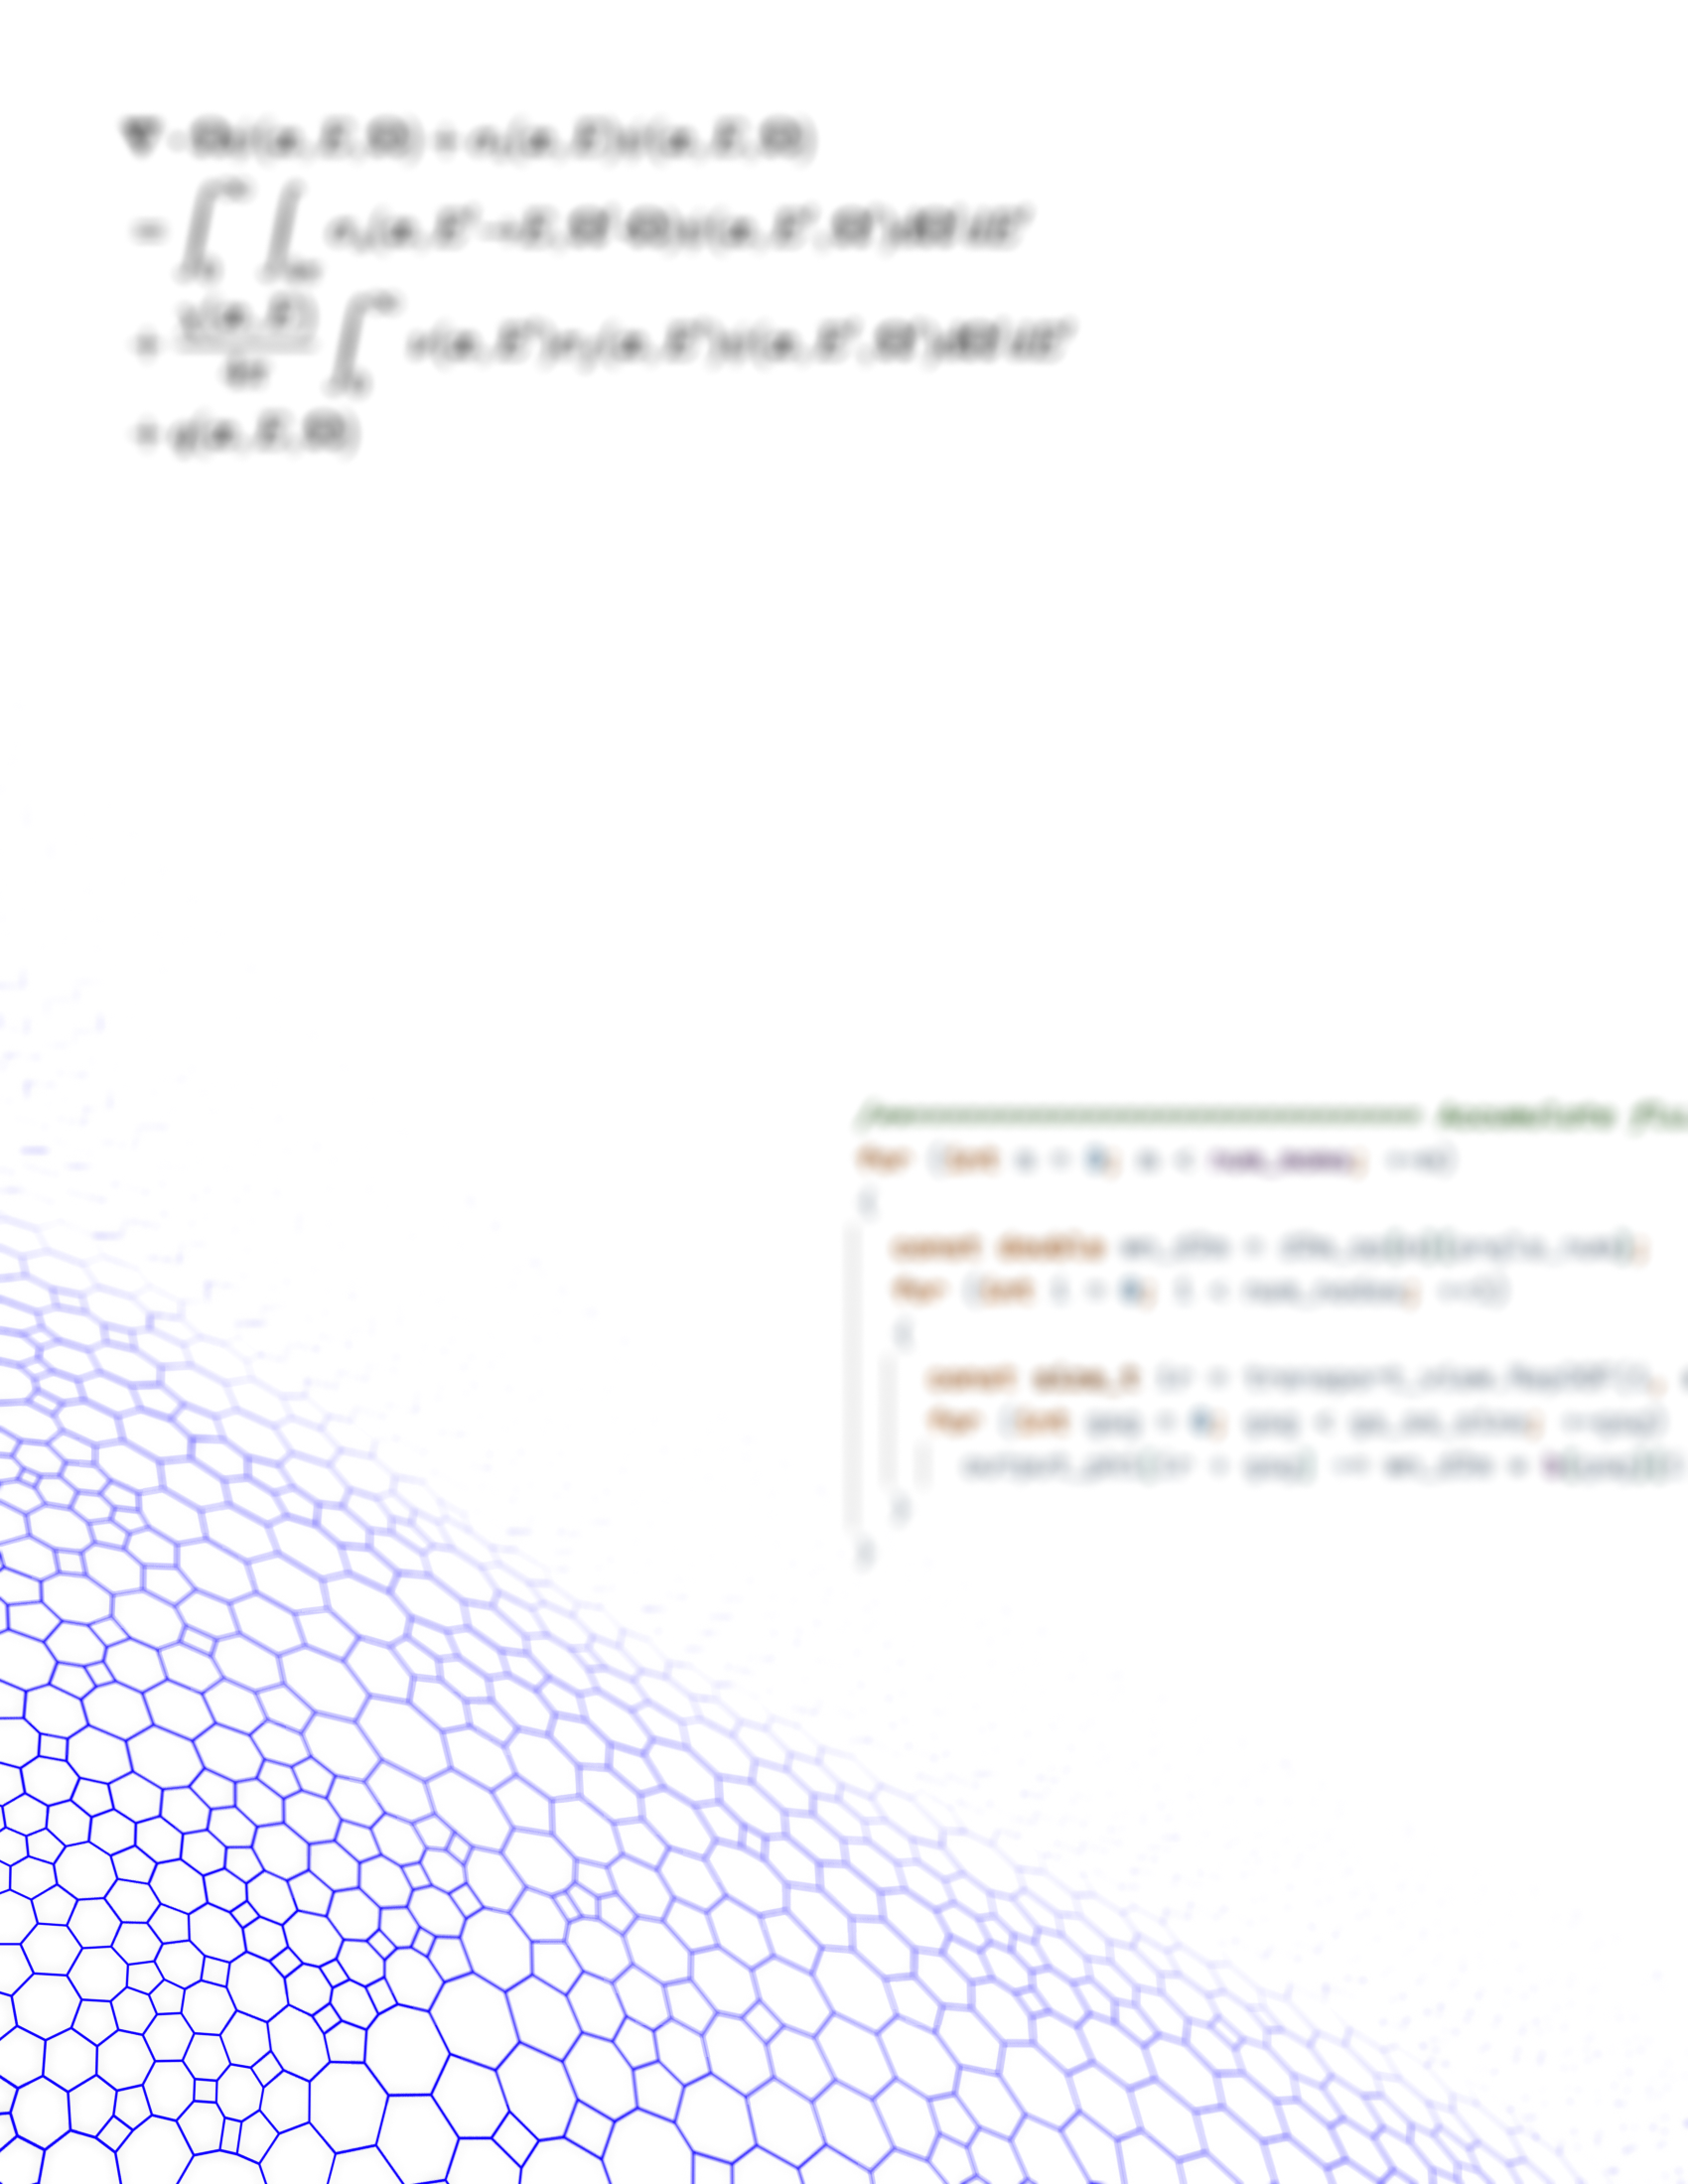
\includegraphics[width=\paperwidth,height=\paperheight,%
			keepaspectratio]{WhitepageBackground.png}%
			\vfill
}}}

%
% Command to make a link back to TOC
%
\newcommand{\BackToTOC}{\hyperlink{toc}{\scriptsize{\color{blue}Back to TOC}}\newline}


\begin{document}
	
\begin{titlepage}
	\AddToShipoutPicture*{\BackgroundPic}
%	\begin{center}
	{\centering 
		\vspace*{3cm}
		{\LARGE\textbf{\DOCSUBJT}}
		
		{\LARGE\textbf{\DOCTITLE}}
		
		\vspace{1cm}
		{\Large \DOCDATE \ \ \DOCREV}
		
		\vspace{1cm}
		{\Large Jan I.C. Vermaak${^{1,2}}$}
		
		\vspace{0.25cm}
		\noindent\rule{\textwidth}{1pt}
		{\small $^1$Idaho National Laboratory, Idaho Falls, Idaho, USA.}
		{\small $^2$Center for Large Scale Scientific Simulations, Texas A\&M Engineering Experiment Station, College Station, Texas, USA.}
		

%	\end{center}



}
\end{titlepage}

\pagestyle{plain}
%\rfoot{Page \thepage \ of \pageref{LastPage}}
\cfoot{\thepage}
%\lfoot{}
%\rhead{}
%\chead{\currentname}
%\lhead{}
%\renewcommand{\footrulewidth}{0.4pt}
%\setlength{\headheight}{13.59999pt}

\pagenumbering{roman}
\chead{Abstract}
\section*{Abstract}\label{abstract}
\addcontentsline{toc}{section}{\nameref{abstract}}


Implementation details of Point-Reactor Kinetics in ChiTech.
\newline
\newline\noindent
\textbf{Keywords:} point-reactor kinetics, transient analysis, implicit, explicit, crank-nicolson

\newpage

\chead{Table of contents}

\tableofcontents
\addtocontents{toc}{~\hfill\textbf{Page}\par \protect\hypertarget{toc}{}}

%
\listoffigures
%%\listoftables





\newpage

\pagestyle{fancy}
\rfoot{Page \thepage \ of \pageref{LastPage}}
\cfoot{}
\lfoot{\truncate{14cm}{\DOCTITLE}}
\rhead{}
\chead{\currentname}
\lhead{}
\renewcommand{\footrulewidth}{0.4pt}
\setlength{\headheight}{13.59999pt}

\pagenumbering{arabic}
%\setcounter{secnumdepth}{3}

\chead{The Point-Reactor Kinetics Equations}
\section{The Point-Reactor Kinetics Equations}\BackToTOC
The Point-Reactor Kinetics (PRK) equations are as follows
\begin{equation}
	\begin{aligned}
		\frac{dn}{dt} = \frac{\beta_{eff} ( \rho (t) - 1)}{\Lambda_0}  n(t) + 
		\sum_{j=0}^{J-1} \lambda_j c_j (t) + s_{ext}(t)
	\end{aligned}
\end{equation}
\begin{equation}
	\begin{aligned}
		\frac{dc_j(t)}{dt} = -\lambda_j c_j(t) + \frac{\beta_{j}}{\Lambda_0} n(t)
	\end{aligned}
\end{equation}
where the time-dependent unknowns are; the neutron population, $n$, and each of the delayed neutron precursor concentrations, $c_j, j=0,...,J-1$. $J$ is total number of precursors. The following are constants; the precursor decay constants [$s^{-1}$], $\lambda_j$, the precursor delayed neutron fractions, $\beta_j$, the total delayed neutron fraction $\beta_{eff} = \sum_{j=0}^{J-1}\lambda_j$, and the neutron generation time $\Lambda_0$ [$s^{-1}$]. The following are known time-dependent variables; the reactivity, $\rho$, in dollar-$\$ $ units, and the external source, $s_{ext}$.


\subsection{Operator form}
From the equations above we devise an operator form by defining
\begin{equation*}
\begin{aligned}
	\mathbf{x} = 
	\begin{bmatrix}
		n \\
		c_0 \\
		\vdots \\
		c_{J-1}
	\end{bmatrix}
	A = 
	\begin{bmatrix}
		\frac{\beta_{eff} ( \rho (t) - 1)}{\Lambda_0} & \lambda_0 & \dots & \dots & \lambda_{J-1} \\
		\frac{\beta_{0}}{\Lambda_0} & -\lambda_0 & 0 & \dots & 0\\ 
		\frac{\beta_{1}}{\Lambda_0} & 0 & \ddots &   & \vdots\\
		\vdots & & & \ddots \\
		\frac{\beta_{J-1}}{\Lambda_0} & 0 &\dots & \dots & -\lambda_{J-1}
	\end{bmatrix}
	\mathbf{q} = 
	\begin{bmatrix}
		s_{ext} \\
		0 \\
		\vdots \\
		0
	\end{bmatrix}
\end{aligned}
\end{equation*}
\begin{equation}
	\frac{d\mathbf{x}}{dt} = A \mathbf{x} + \mathbf{q}
\end{equation}

\subsection{Time stepping schemes}
There is currently only three time stepping schemes available, they are: \newline
{\ttfamily explicit\_euler, crank\_nicolson, implicit\_euler}.
\subsubsection{{\ttfamily explicit\_euler}}
For explicit Euler timestepping the operator form of our equation becomes
\beqn 
\frac{1}{\Delta t} (\mathbf{x}^{t+1} - \mathbf{x}^t) &= A \mathbf{x}^t + \mathbf{q} \\
\therefore \mathbf{x}^{t+1} &= \mathbf{x}^t + \Delta t A \mathbf{x}^t + \Delta t \mathbf{q}
\eeqn 
\subsubsection{{\ttfamily crank\_nicolson, implicit\_euler}, $\theta$-scheme time stepping}
{\ttfamily crank\_nicolson, implicit\_euler} can both be represented using a $\theta$-scheme, i.e., $\theta = \frac{1}{2} \to ${\ttfamily crank\_nicolson} and $\theta = 1 \to ${\ttfamily implicit\_euler}.


For $\theta$-scheme time stepping, we have
\begin{equation}
	\frac{1}{\Delta t} (\mathbf{x}^{t+1} - \mathbf{x}^t) = A(\theta \mathbf{x}^{t+1} + (1-\theta) \mathbf{x}^{t}) + \mathbf{q}
\end{equation}
for which can make the convenient manipulation
\begin{equation}
\begin{aligned}
	\mathbf{x}_{\theta} &= \theta \mathbf{x}^{t+1} + (1-\theta) \mathbf{x}^{t} \\
	\therefore \mathbf{x}^{t+1} &= \mathbf{x}^t + \frac{1}{\theta} (\mathbf{x}_\theta - \mathbf{x}^t),
\end{aligned}
\end{equation}
then we plug the expression for $\mathbf{x}^{t+1}$ into eq. 1.4, to get
\begin{equation}
	\tau (\mathbf{x}_\theta - \mathbf{x}^t) = A\mathbf{x}_\theta  + \mathbf{q}
\end{equation}
where $\tau = \frac{1}{\theta \Delta t}$ and which can be arranged into implicit form as
\begin{equation}
	(I - \frac{1}{\tau}A)\mathbf{x}_{\theta} = \mathbf{x}^t + \frac{1}{\tau} \mathbf{q}
\end{equation}
which in turn can be written as a linear system
\begin{equation}
	A_{\theta} \mathbf{x}_{\theta} = \mathbf{b}_{\theta}
\end{equation}
where
\beqn
A_\theta = (I - \frac{1}{\tau}A)
\eeqn 
and
\beqn 
\mathbf{b}_{\theta} = \mathbf{x}^t + \frac{1}{\tau} \mathbf{q}
\eeqn 

At each time step we solve the system in eq. 1.8 to get $\mathbf{x}_\theta$, thereafter we update 
\beqn 
\mathbf{x}^{t+1} &= \mathbf{x}^t + \frac{1}{\theta} (\mathbf{x}_\theta - \mathbf{x}^t)
\eeqn 

\subsection{Initialization}
With an external source and $\rho < 0$ we can initialize the problem because there is a unique solution. The solution is then
\beqn 
\mathbf{x}^0  = A^{-1} \mathbf{q}.
\eeqn 
Otherwise we initialize the problem with $\rho = 0$ and $s_{ext} = 0$ as
\beqn 
A: \text{ row 0 } = [1, 0, ..., 0] \to A_{temp} \\
\mathbf{b}_{temp} = [1, 0, ..., 0]\\
\mathbf{x}^0 = A_{temp}^{-1} \mathbf{b}_{temp}
\eeqn 

\newpage
\begin{thebibliography}{1}
	
	\bibitem{Ragusa NUEN618 slides} Ragusa J.C., {\em NUEN-618 slides} 2020.
	   
\end{thebibliography}

\newpage
\begin{appendices}
\section{First appendix}
Put ``Lazy reader stuff here".
\end{appendices}

\end{document}